\newcommand{\posterPolarPrinciples}[1]{

\setlength{\frameWidth}{#1}
\setlength{\unitlength}{0.02\frameWidth}
\psset{unit=\unitlength}

\rput[tl](2.5,18){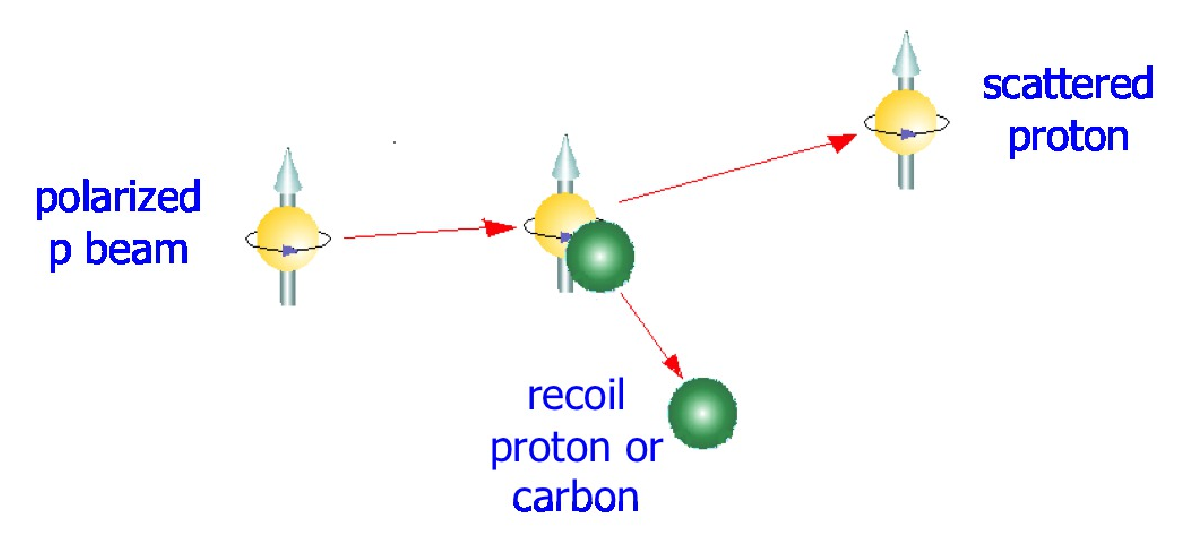
\includegraphics[width=30\unitlength]{graphics/elastic}}

\rput[tl](1,30) {%
\begin{minipage}{45\unitlength}

\raggedright

\begin{list}{\labelitemi}{\setlength{\itemsep}{2mm}
                          \setlength{\topsep}{0mm}}

   \item Fixed targets are used to measure proton beam polarization

   \begin{list}{\labelitemii}{\setlength{\itemsep}{3mm}
                             \setlength{\topsep}{0mm}}

      \item {\bf H-jet polarimeter}

      \small
      \begin{list}{\labelitemiii}{\setlength{\itemsep}{3mm} \setlength{\topsep}{3mm}}
         \item Vertical hydrogen jet target $\sim 6-7$~mm in diameter
      \end{list}
      \normalsize

      \item {\bf p-Carbon polarimeters}

      \small
      \begin{list}{\labelitemiii}{\setlength{\itemsep}{3mm} \setlength{\topsep}{3mm}}
         \item Ultra thin carbon ribbon $2.5~\text{cm} \times 10~\mu\text{m} \times 25~\text{nm}$
         \item Vertical and horizontal targets
      \end{list}
      \normalsize
   \end{list}

\end{list}

\end{minipage}
}

\rput[t](42,28){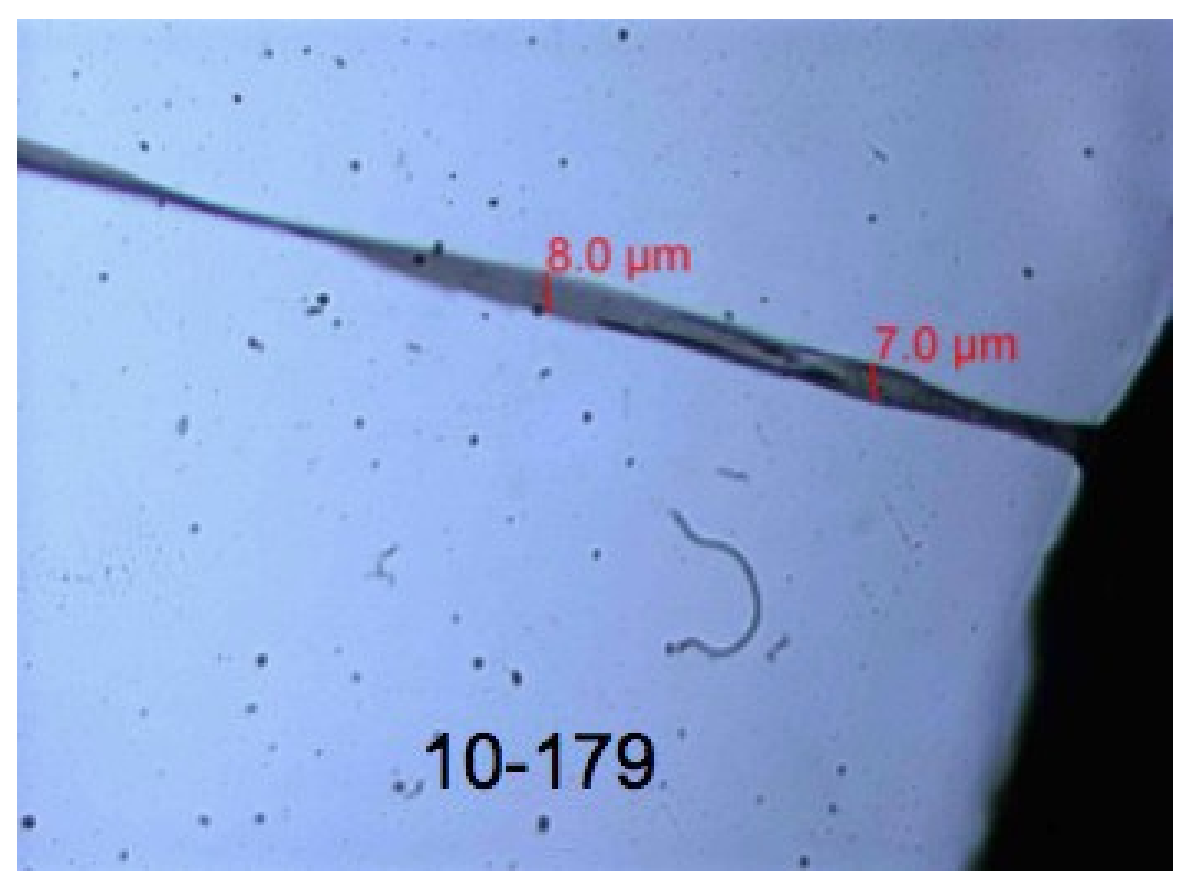
\includegraphics[width=14\unitlength]{graphics/target}}

\psline[linewidth=0.1,linecolor=blueDark](34,5)(34,18)

\rput[tl](35.5,16){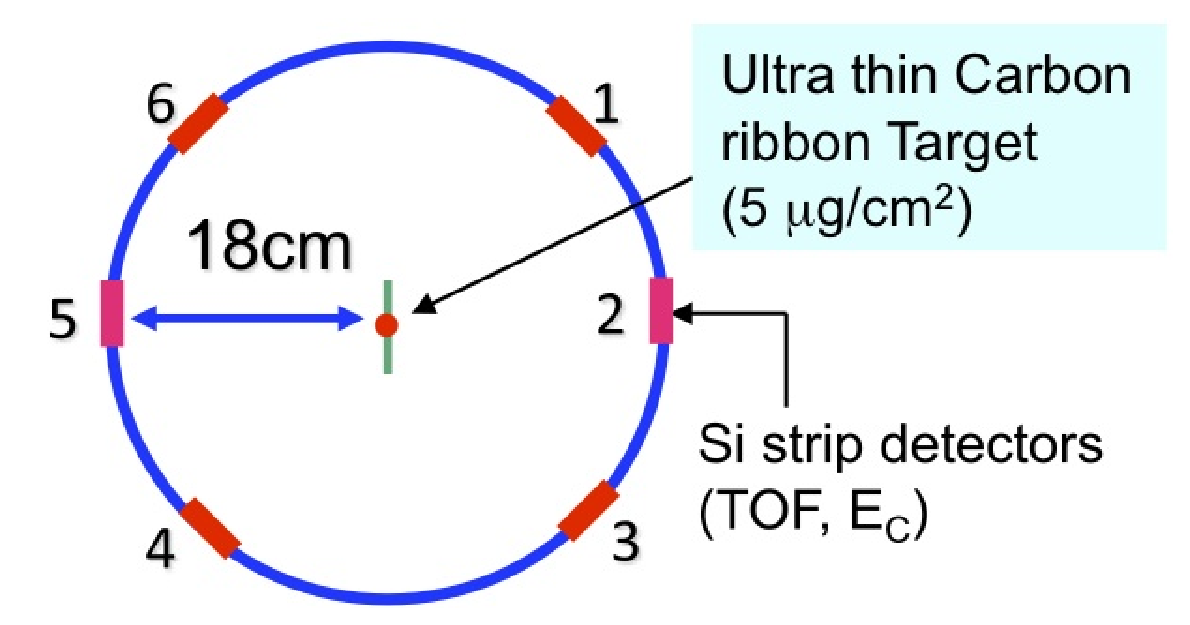
\includegraphics[width=20\unitlength]{graphics/pcarbon_det}}


\rput[tl](1,4) {%
\begin{minipage}{47\unitlength}

\begin{list}{\labelitemi}{\setlength{\itemsep}{0\unitlength}
                          \setlength{\topsep}{0mm}}

   \item \textbf{Measured polarization is:}
   \psframebox{\normalsize  $P = \frac{1}{A_N} \times \frac{N_L - N_R}{N_L + N_R}$},
   \small where $A_N$ is small~$\sim~3$~\%

   \normalsize
   \item No need to know $A_N$ with Hydrogen Jet polarimeter

\end{list}

\end{minipage}
}


%\rput{0}{\psgrid[gridlabels=0.7,subgriddiv=0, griddots=3](1,-1)(0,0)(\myPsPictureWidthLocal,\myPsPictureHeightLocal)}

}

\setlength{\unitlength}{10mm}
\psset{unit=\unitlength}
